\chapter{Improving the Way Neural Networks Learn}

\section{The Cross-Entropy Cost Function}

\begin{exercise}
Show that the cross-entropy function is minimized when $\sigma(z) = y$ for all inputs.
\end{exercise}
\begin{solution}
The cross-entropy function is defined as:
\[
    C = - \frac{1}{m} \sum_{i = 1}^m [y_i \ln (a_i) + (1 - y_i) \ln (1 - a_i)],
\]
where the $y_i$s are fixed and the $a_i$s are the ``variables.'' Now $\partial C / \partial a_i$
is given by:
\[
    \frac{\partial C}{\partial a_i} = \frac{1}{m} \frac{a_i - y_i}{a_i (1 - a_i)}. 
\]
At an extremum point of $C$, each component of the gradient $\nabla_a C$ will be zero. This 
happens when $a_i = y_i$ for all~$1 \leq i \leq m$. 

As a side note, the function $H(y) = - [y \ln(y) + (1 - y) \ln (1 - y)]$ for $y \in (0, 1)$ 
is called the binary entropy function and behaves as shown in Figure~\ref{fig:binary_entropy}. 
\end{solution}

\begin{figure}[ht]
\begin{center}
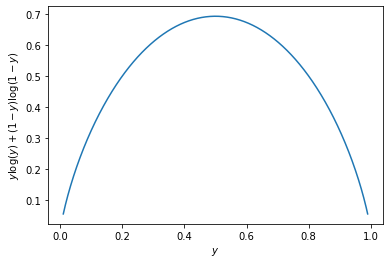
\includegraphics[scale=0.60]{entropy.png}
\end{center}
\caption{The Binary Entropy Function}
\label{fig:binary_entropy}
\end{figure}

\begin{exercise}
Partial derivatives of the cross-entropy cost function in multi-layer
networks.
\end{exercise}
\begin{solution}
The cross-entropy function for a single training example~$x$ for the last
layer~$L$ of the network is defined as:
\[
    C(x) = - \sum_j \left [ y_j \ln (a_j^L) + (1 - y_j) \ln(1 - a_j^L) \right ],
\]
where the sum is over all neurons~$j$ in layer~$L$. To recap notation,  
\[
a_j^L = \sigma(z_j^L) = \sum_k w_{j k}^L a_k^{L - 1} + b_j^L.
\]
For this training example~$x$,
\begin{align*}
    \frac{\partial C(x)}{\partial z_j^L} 
        & = - \frac{y_j}{a_j^L} \cdot \sigma' (z_j^L) + \frac{1 - y_j}{1 - a_j^L} \cdot \sigma' (z_j^L) \\
        & = \frac{-y_j + y_j a_j^L + a_j^L - y_j a_j^L}{a_j^L (1 - a_j^L)} \cdot \sigma' (z_j^L) \\
        & = a_j^L - y_j.
\end{align*}
The last equality follows since $\sigma' (z_j^L) = a_j^L (1 - a_j^L)$.

Again, for this single training example~$x$, $\partial C (x) / \partial w_{j k}^L$ 
is given by:
\begin{align*}
    \frac{\partial C (x)}{\partial w_{j k}^L} 
        & = \frac{\partial C}{\partial z_j^L} \cdot \frac{\partial z_j^L}{\partial w_{j k}^L} \\
        & = (a_j^L - y_j) \cdot a_k^{L - 1}. 
\end{align*}
For $n$ training examples, the cost function is defined as $\frac{1}{n} \sum_{x} C(x)$ and 
this derivative is: 
\[
    \frac{\partial C}{\partial w_{j k}^L} = \frac{1}{n} \sum_x a_k^{L - 1} (a_j^L - y_j).
\]
If we were to replace $C(x)$ by the usual quadratic cost $\frac{1}{2}(y_j - a_j^L)^2$, then 
the same derivative would have been:
\[
    \frac{1}{n} \sum_x a_k^{L - 1} (a_j^L - y_j) \cdot \sigma' (z_j^L).
\]
\end{solution}

\subsection{Deriving the Cross-Entropy Function}

Given a single neuron with $r$ input weights $w_1, \ldots, w_r$ and bias~$b$,
and a single input $\vect{x} = \trans{(x_1, \ldots, x_r)}$, we would like the
cost function $C$ to depend on the weights and the bias as follows:
\begin{align}
    \frac{\partial C}{\partial w_j} & = x_j (a - y) \\
    \frac{\partial C}{\partial b}   & = a - y, \label{eqn:cost_bias}
\end{align}
where $a = \sigma(\sum_{j} w_j x_j + b)$ and $y$ is the desired output 
corresponding to $\vect{x}$. 

Using the chain rule, we obtain:
\begin{align}
    \frac{\partial C}{\partial b} & = 
        \frac{\partial C}{\partial a} \cdot 
        \frac{\partial a}{\partial z} \cdot 
        \frac{\partial z}{\partial b} \nonumber \\
        & = \frac{\partial C}{\partial a} \cdot \sigma'(z) \nonumber \\ 
        & = \frac{\partial C}{\partial a} \cdot a (1 - a) \label{eqn:cross_entropy} 
\end{align}
From equations~(\ref{eqn:cost_bias} and~\ref{eqn:cross_entropy}), we obtain:
\[
    \frac{\partial C}{\partial a} = \frac{a - y}{a (1 - a)} = 
        \frac{1}{1 - a} - y \left ( \frac{1}{1 - a} + \frac{1}{a}\right ).
\]
Integrating both sides wrt~$a$, we obtain:
\[
    C = - [(1 - y) \ln (1 - a) + y \ln (a)] + \text{ a constant}.
\]

\section{Softmax}

Consider a classification problem, where labelled examples take the form 
$(\vect{x}, \vect{y})$, where $\vect{x} \in \R^m$ and $\vect{y} \in \{0, 1\}^J$ 
denotes to which of the $J$ classes $\vect{x}$ belongs to. 
In such cases, it makes sense to have the last 
layer of the neural network to have $J$ neurons with the softmax activation:
\begin{align*}
    z_j^L & = \sum_k w_{j k}^L a_{k}^{L - 1} + b_j \\
    a_j^L & = \frac{e^{z_j^L}}{ \sum_{i = 1}^J e^{z_i^L}}
\end{align*}

The cost associated with the input $(\vect{x}, \vect{y})$ where $y_r = 1$ 
is defined as the negative log-likelihood of the activation $a_{r}^L$:
\[
    C(\vect{x}, \vect{y}) = - \ln a_{r}^L.
\]

The partial derivatives $\partial C / \partial b_j^L$ and   $\partial C / \partial w_{j k}^L$
can be computed easily as follows. Depending on whether the index $j$ and the class index~$r$
are the same or not, we have two cases for each partial derivative.
\begin{align}
    \frac{\partial C}{\partial b_{r}^L} 
        & =   - \frac{1}{a_{r}^L} \cdot 
            \left [ \frac{e^{z_{r}^L}}{ \sum_{i = 1}^J e^{z_i^L}} - 
                    \left ( \frac{e^{z_{r}^L}}{ \sum_{i = 1}^J e^{z_i^L}} \right )^2 
            \right ] = - 1 + a_{r}^L \\
\frac{\partial C}{\partial b_j^L} 
      & = 
    - \frac{1}{a_{r}^L} \cdot \left [ 0 - \frac{e^{z_{r}^L} e^{z_j^L}}{ \left ( \sum_{i = 1}^J e^{z_i^L} \right )^2} 
                            \right ] = a_j^L. 
\end{align}
The first equation is when the index $r = j$ and the second when $r \neq j$. 
These two expressions can be summarized into one: 
\begin{equation}
\frac{\partial C}{\partial b_j^L} = a_{j}^L - y_j.
\end{equation}

Similarly, the partial derivative expression for  $\partial C / \partial w_{j k}^L$
can be written as:
\begin{equation}
\frac{\partial C}{\partial w_{j k}^L} = a_{k}^{L - 1} \cdot (a_{j}^L - y_j). 
\end{equation}

\begin{exercise}
Where does the ``softmax'' name come from? Consider the following variant 
of the softmax function:
\[
    a_j^L =  \frac{e^{c z_j^L}}{ \sum_{i = 1}^J e^{c z_i^L}},
\]
where $c$ is a positive constant. What is the limit of $a_j^L$ 
as $c \to \infty$?
\end{exercise}
\begin{solution}
Let $z_r^L = \max_i \{z_i^L\}$. We could then write the modified softmax
function as:
\[
    a_j^L =  \frac{e^{c (z_j^L - z_r^L)}}{ 1 + \sum_{i \neq r} e^{c (z_i^L - z_r^L)}}. 
\]
If $j = r$, then the numerator is $1$ and the denominator approaches $1$ as $c \to \infty$
and $a_j^L \to 1$. On the other hand, if $j \neq r$, the numerator $\to 0$ as $c \to \infty$;
the denominator in any case approaches~$1$ and hence~$a_j^L \to 0$. The point here is 
that $a_j^L = 1$ if $z_j^L$ is the maximum and $a_j^L = 0$ otherwise. 
\end{solution}

\section{Regularization}

Regularization is a set of methods used to prevent overfitting and improve 
generalization performance. The typical way to do this is to tack on a 
``regularization term'' in the loss function. The most commonly used of these 
are the $L_1$-regularization and the 
$L_2$-regularization. These are defined in terms of the $L_1$ and $L_2$-norms 
respectively. For a real $p \geq 1$, the $L_p$-norm of a vector $w \in \R^d$ is defined as  
\begin{equation}
    \norm{w} = \left ( |w_1|^p + \cdots + |w_d|^p \right )^{1/p}.
\end{equation}
Let us assume that $\mathscr{L}(w)$ is the original loss function. Then the 
$L_2$-regularized loss functions looks like this:
\[
    \mathscr{L}(w) + \frac{\alpha}{2} \cdot \norm{w}_2^2,
\]
where $\alpha > 0$ is real number that specifies the ``strength'' of the 
regularization. 

\subsection{$L_2$-regularization Analysis}
Let $w^{\star}$ be an optimal solution to $\mathscr{L}(w)$, the unregularized 
loss function. Given a vector $w \in \R^{d}$, write $w$ as $w^{\star} + \epsilon$, 
where $\epsilon$ is viewed as the ``error.'' Use a second-order Taylor series  
expansion to write down the loss~$\mathscr{L}$ at the point $w^{\star} + \epsilon$ 
as:
\begin{equation}
\label{eqn:loss_taylor_series}
\mathscr{L}(w^{\star} + \epsilon) = 
    \mathscr{L}(w^{\star}) + 
    \epsilon^{T} \cdot \nabla \mathscr{L}(w^{\star}) +
    \frac{1}{2} \epsilon^{T} \cdot H_{\mathscr{L}} \cdot \epsilon,
\end{equation}
where $H_{\mathscr{L}}$ represents the Hessian of $\mathscr{L}$ evaluated at 
$w^{\star}$. Recall that the Hessian, in this case, is a $d \times d$ matrix 
whose $(i, j)$th term is given by:
\[
    \left . \frac{\partial^2 \mathscr{L}(w)}{\partial w_i \partial w_j} \right |_{w^{\star}}.
\]
We assume that the loss function is continuous at $w^{\star}$ so that the order 
of partial derivatives does not matter. In this case, the Hessian is a symmetric 
$d \times d$ matrix. In particular, note that this implies that all eigenvalues 
of the Hessian matrix are real. 

Since $\nabla \mathscr{L}(w^{\star}) = 0$, we may rewrite 
Equation~\ref{eqn:loss_taylor_series} as:
\[
    \mathscr{L}(w) = \mathscr{L}(w^{\star}) + 
    \frac{1}{2} (w - w^{\star})^{T} \cdot H_{\mathscr{L}} \cdot (w - w^{\star}).
\]
Taking gradients wrt~$w$, we obtain that:
\begin{equation}
\label{eqn:loss_func_grad}
    \nabla \mathscr{L}(w) = 0 + H_{\mathscr{L}} \cdot (w - w^{\star}).
\end{equation}

Consider the $L_2$-regularized loss function 
$\tilde{\mathscr{L}}(w) = \mathscr{L}(w) + \frac{\alpha}{2} \cdot \norm{w}^2$ .
Let $\tilde{w}$ be an optimum solution to this regularized loss function. Then 
\begin{equation}
\label{eqn:reg_loss_func_grad}
    0 = \nabla \tilde{\mathscr{L}}(\tilde{w}) = 
        \nabla \mathscr{L}(\tilde{w}) 
        + \alpha \tilde{w}.
\end{equation}
Using the expression from Equation~\ref{eqn:loss_func_grad} in the above equation, 
we get:
\begin{gather}
H_{\mathscr{L}} \cdot (\tilde{w} - w^{\star}) + \alpha \tilde{w} = 0 \notag \\
\begin{split}
(H_{\mathscr{L}} + \alpha \cdot I) \tilde{w} & = H_{\mathscr{L}} \cdot w^{\star} \\
\therefore \tilde{w} & = (H_{\mathscr{L}} + \alpha \cdot I)^{-1} \cdot H_{\mathscr{L}} \cdot w^{\star}.
\end{split}
\end{gather}
Here we are assuming that the symmetric matrix $H_{\mathscr{L}} + \alpha \cdot I$
is invertible. In fact, we are going make a stronger assumption about $H_{\mathscr{L}}$
that it is positive definite. Recall that this means that the eigenvalues of 
$H_{\mathscr{L}}$ are all strictly positive. 

Any symmetric matrix $A$ of order~$d$ can be written as $A = Q \Lambda Q^{T}$, 
where the columns of $Q$ are the eigenvectors $q_1, \ldots, q_d$ of $A$ and 
$\Lambda = \diag(\lambda_1, \ldots, \lambda_d)$, where $A q_i = \lambda_i q_i$.
Moreover, the eigenvectors $q_1, \ldots, q_d$ form an orthonormal basis of $\R^{d}$. 
In particular, this means that $Q^{T}Q = I$ so that $Q^{-1} = Q^{T}$. Substituting 
this \textbf{spectral decomposition} form for $H_{\mathscr{L}}$ in the last 
equation for $\tilde{w}$, we get:
\begin{align}
    \label{eqn:optimal_regularized_solution}
    \tilde{w} 
        & = (H_{\mathscr{L}} + \alpha I)^{-1} \cdot H_{\mathscr{L}} \cdot w^{\star} \nonumber \\ 
        & = (Q \Lambda Q^{T} + \alpha Q I Q^{T})^{-1} \cdot Q \Lambda Q^{T} \cdot w^{\star} \nonumber \\
        & = (Q (\Lambda + \alpha I )Q^{T})^{-1} \cdot Q \Lambda Q^{T} \cdot w^{\star} \nonumber \\
        & = Q (\Lambda + \alpha I)^{-1} Q^{T} \cdot Q \Lambda Q^{T} \cdot w^{\star} \nonumber \\
        & = Q (\Lambda + \alpha I)^{-1} \Lambda Q^{T} \cdot w^{\star} \nonumber \\
        & = Q 
            \diag \left ( \frac{\lambda_1}{\lambda_1 + \alpha}, \ldots, \frac{\lambda_d}{\lambda_d + \alpha} \right ) 
            Q^{T} \cdot w^{\star}.
\end{align} 

This can be interpreted as follows. To obtain an optimal solution~$\tilde{w}$ to 
the $L_2$-regularized problem, one proceeds as follows. One takes an optimal solution~$w^{\star}$ 
to the unregularized loss function, applies an orthogonal transformation $Q^{T}$ 
to it which has the effect of rotating it. Each component of that rotated vector 
is then scaled by the matrix 
$\diag(\lambda_1 / (\lambda_1 + \alpha), \ldots, \lambda_d / (\lambda_d + \alpha))$. But 
the scaling for component~$i$ equals $\lambda_i / (\lambda_i + \alpha)$ which 
depends on the eigenvalue~$\lambda_i$. If $\lambda_i \gg \alpha$, then the 
fraction $\lambda_i / (\lambda_i + \alpha) \approx 1$ and there 
is no appreciable change in that component. But if $\lambda_i \ll \alpha$, then 
$\lambda_i / (\lambda_i + \alpha) \approx 0$ and that component effectively zeros 
out. Finally, a reverse orthogonal transform is applied to the scaled 
vector. Had the diagonal entries of the scaling matrix above been all the same, 
the effect would be to simply multiply $w^{\star}$ by this scaling factor. But 
different eigenvalues imply a different scaling for each component. 
In the end, the eigenvalues of $H_{\mathscr{L}}$ determine which components 
of the weight vector~$w$ are important.

\subsection{Other Methods for Regularizing Neural Nets}
Other than constrain the loss function, there are several other practical techniques
to regulaize neural networks. These are:
\begin{enumerate}
    \item Early stopping
    \item Dataset augmentation
    \item Noise injection
    \item Dropout.
\end{enumerate}

\subsubsection{Early stopping}
The ideas here is to continuously monitor the loss function and stop the training
when the validation loss does not meet some previously defined criterion. An 
example of such a criterion is the \emph{error change criterion}: pause 
training when the validation error does not drop over a window of, say, 10 epochs; 
continue training for a fixed number of epochs when this criterion is reached 
before finally stopping. 

Another idea is the \emph{weight change criterion}: compare the weights at epochs, 
say,  $t - 10$ and~$t$ and test whether
\[
    \max_{i} \norm{w_i^{(t - 10)} - w_i^{(t)}} \le \rho,
\]  
where $\rho$ is some predefined threshold. Instead of using an absolute value, 
one could use a threshold based on the percentage of the weight $w_i^{t}$.

\subsubsection{Dataset Augmentation}
This idea is particularly relevant when using neural networks to detect images. 
Certain transformations of an image do not change the label of the image. These 
include distorting or blurring the image, rotating it, changing its color, 
injecting noise, mirroring it, and so on and so forth. Using these transformations, 
one gets to increase the size of the training dataset. This has the effect of 
preventing overfitting as the neural network is exposed to data that is not 
explicitly present in the original dataset.

Another method of data augmentation is that of \emph{mix up}. This consists in 
first choosing a parameter $\lambda \in [0, 1]$, and then given a pair of data points
$(x^{(i)}, y^{(i)})$ and $(x^{(j)}, y^{(j)})$, creating a new data point 
$(\tilde{x}, \tilde{y})$, which is the convex combination of these data points:
\begin{align}
    \tilde{x} & = \lambda x^{(i)} + (1 - \lambda) x^{(j)} \\
    \tilde{y} & = \lambda y^{(i)} + (1 - \lambda) y^{(j)}.
\end{align}    

\subsubsection{Noise Injection}
Here the idea is to add noise to either the input data or the labels or the 
gradients during training. Let's look at the case where one adds Gaussian 
noise to the input data during training when the loss function is the 
expected squared-loss. 

As usual, let the data points be 
$(x, y) \in \R^{d} \times \R$ and let us assume that the joint density 
of the input-output pairs is given by the function 
$f_{X, Y} \colon \R^{d} \times \R \to [0, 1]$ . Let us add Gaussian noise 
$\epsilon \sim N_d(0_d, \Sigma_d)$, where $0_d$ is the zero-vector 
from $\R^d$ and $\Sigma_d = \diag(\sigma^2, \ldots, \sigma^2)$. Recall that 
if a random vector has a multivariate normal distribution, then two components
of that vector are independent iff they are uncorrelated. This is \emph{not} 
true for random variables $X, Y$, in general, even if both are normally distributed. 
In this specific case, this implies that for all $1 \leq i, j \leq d$: 
\begin{equation}
    \Expone{ \epsilon_i \epsilon_j }= 
    \left \{ \begin{array}{ll} 
                0        & \quad \text{ if } i \neq j \\
                \sigma^2 & \quad \text{ if } i = j. 
              \end{array}
    \right .
\end{equation}

The expected squared-loss is:
\begin{equation}
    \loss (w) = \Exptwo{(x, y) \sim f_{X, Y}}{(w^T x - y)^2}  
              = \iint (w^T x - y)^2 \cdot f_{X, Y}(x, y) \dx y \dx x.
\end{equation}
The expected squared-loss error in the presence of noise is given by:
\begin{align}
    \label{eqn:loss_with_noise}
    \tilde{\loss} (w) 
        & = \Exptwo{\epsilon \sim N_d, (x, y) \sim f_{X, Y}}{(w^T (x + \epsilon) - y)^2} \nonumber \\ 
        & = \iint \Exptwo{\epsilon \sim N_d}{(w^T (x + \epsilon) - y)^2 \mid (x, y)} \cdot f_{X, Y}(x, y) \dx y \dx x.
\end{align}

Simplifying the expression for the loss in Equation~(\ref{eqn:loss_with_noise}), we get
that:
\begin{align}
    \label{eqn:loss_with_noise_simple}
    \tilde{\loss} (w) 
        & = \iint \Exptwo{\epsilon \sim N_d}{ (w^T x - y)^2 + 
                           2(w^T x - y) (w^T \epsilon) + 
                           (w^T \epsilon)^2 
                           \mid (x, y)} 
                   f_{X, Y}(x, y) \dx y \dx x \nonumber \\
        & = \iint \left [ (w^T x - y)^2 + 2(w^T x - y) \Expone{(w^T \epsilon) \mid (x, y)} + 
                          \Expone{(w^T \epsilon)^2 \mid (x, y)} \right ] f_{X, Y}(x, y) \dx y \dx x   
\end{align}

The expectations inside the integral sign in the above equation are all wrt the 
distribution of $\epsilon$. Now, 
\begin{align}
    \label{eqn:noise_mean}
    \Exptwo{\epsilon \sim N_d}{(w^T \epsilon) \mid (x, y)} 
        & = \Exptwo{\epsilon \sim N_d}{(w^T \epsilon)} \nonumber \\
        & = \Exptwo{\epsilon \sim N_d}{w_1 \epsilon_1 + \cdots + w_d \epsilon_d} \nonumber \\
        & = 0.
\end{align}
Moreover, 
\begin{align}
    \label{eqn:noise_variance}
    \Exptwo{\epsilon \sim N_d}{(w^T \epsilon)^2 \mid (x, y)} 
        & = \Exptwo{\epsilon \sim N_d}{(w^T \epsilon)^2} \nonumber \\
        & = \Exptwo{\epsilon \sim N_d}{\sum_{i = 1}^{d} w_i^2 \epsilon_i^2 + 
                    2 \cdot \sum_{i < j} w_i w_j \epsilon_i \epsilon_j} \nonumber \\
        & = \sum_{i = 1}^{d} w_i^2 \sigma^2 \nonumber \\
        & = \sigma^2 \sum_{i = 1}^{d} w_i^2.
\end{align}

From Equations~\ref{eqn:loss_with_noise_simple}, \ref{eqn:noise_mean} 
and~\ref{eqn:noise_variance}, we obtain that:
\begin{equation}
    \tilde{\loss} (w) = \loss (w) + \sigma^2 \sum_{i = 1}^{d} w_i^2,
\end{equation}
which is the expression for the loss function regularized with $L_2$-loss.
